%!TEX TS-program = xelatex
\documentclass[notes,12pt, aspectratio=169]{beamer}

\usepackage{amsmath,amsfonts,amssymb,amsthm,mathtools}  % пакеты для математики
\usepackage{minted}

\usepackage[english, russian]{babel} % выбор языка для документа
\usepackage[utf8]{inputenc} % задание utf8 кодировки исходного tex файла
\usepackage[X2,T2A]{fontenc}        % кодировка

\usepackage{fontspec}         % пакет для подгрузки шрифтов
\setmainfont{Helvetica}  % задаёт основной шрифт документа

% why do we need \newfontfamily:
% http://tex.stackexchange.com/questions/91507/
\newfontfamily{\cyrillicfonttt}{Helvetica}
\newfontfamily{\cyrillicfont}{Helvetica}
\newfontfamily{\cyrillicfontsf}{Helvetica}

\usepackage{unicode-math}     % пакет для установки математического шрифта
% \setmathfont{Neo Euler} % шрифт для математики

\usepackage{polyglossia}      % Пакет, который позволяет подгружать русские буквы
\setdefaultlanguage{russian}  % Основной язык документа
\setotherlanguage{english}    % Второстепенный язык документа

% Шрифт для кода
\setmonofont[Scale=0.85]{Monaco}
\usepackage{verbments}

\usepackage{pgfpages}
% These slides also contain speaker notes. You can print just the slides,
% just the notes, or both, depending on the setting below. Comment out the want
% you want.
%\setbeameroption{hide notes} % Only slide
%\setbeameroption{show only notes} % Only notes
%\setbeameroption{show notes on second screen=right} % Both

\usepackage{array}

\usepackage{tikz}
\usepackage{verbatim}
\setbeamertemplate{note page}{\pagecolor{yellow!5}\insertnote}
\usetikzlibrary{positioning}
\usetikzlibrary{snakes}
\usetikzlibrary{calc}
\usetikzlibrary{arrows}
\usetikzlibrary{decorations.markings}
\usetikzlibrary{shapes.misc}
\usetikzlibrary{matrix,shapes,arrows,fit,tikzmark}

\usepackage{hyperref}
\usepackage{lipsum}
\usepackage{multimedia}
\usepackage{multirow}
\usepackage{dcolumn}
\usepackage{bbm}
\newcolumntype{d}[0]{D{.}{.}{5}}

\usepackage{changepage}
\usepackage{appendixnumberbeamer}
\newcommand{\beginbackup}{
   \newcounter{framenumbervorappendix}
   \setcounter{framenumbervorappendix}{\value{framenumber}}
   \setbeamertemplate{footline}
   {
     \leavevmode%
     \hline
     box{%
       \begin{beamercolorbox}[wd=\paperwidth,ht=2.25ex,dp=1ex,right]{footlinecolor}%
%         \insertframenumber  \hspace*{2ex} 
       \end{beamercolorbox}}%
     \vskip0pt%
   }
 }
\newcommand{\backupend}{
   \addtocounter{framenumbervorappendix}{-\value{framenumber}}
   \addtocounter{framenumber}{\value{framenumbervorappendix}} 
}

% для имитации питоновского синтаксиса 
\newcommand{\pgr}[1]{{\color{green} \textbf{#1}}}


%%%%%%%%%% Работа с картинками %%%%%%%%%
\usepackage{graphicx}                  % Для вставки рисунков
\usepackage{graphics}
\graphicspath{{images/}}    % можно указать папки с картинками
\usepackage{wrapfig}                   % Обтекание рисунков и таблиц текстом

\usepackage[space]{grffile}
\usepackage{booktabs}

% These are my colors -- there are many like them, but these ones are mine.
\definecolor{blue}{RGB}{0,114,178}
\definecolor{red}{RGB}{213,94,0}
\definecolor{yellow}{RGB}{240,228,66}
\definecolor{green}{RGB}{0,128, 0}

\hypersetup{
  colorlinks=false,
  linkbordercolor = {white},
  linkcolor = {blue}
}


%% I use a beige off white for my background
\definecolor{MyBackground}{RGB}{255,253,218}

%% Uncomment this if you want to change the background color to something else
%\setbeamercolor{background canvas}{bg=MyBackground}

%% Change the bg color to adjust your transition slide background color!
\newenvironment{transitionframe}{
  \setbeamercolor{background canvas}{bg=yellow}
  \begin{frame}}{
    \end{frame}
}

\setbeamercolor{frametitle}{fg=blue}
\setbeamercolor{title}{fg=black}
\setbeamertemplate{footline}[frame number]
\setbeamertemplate{navigation symbols}{} 
\setbeamertemplate{itemize items}{-}
\setbeamercolor{itemize item}{fg=blue}
\setbeamercolor{itemize subitem}{fg=blue}
\setbeamercolor{enumerate item}{fg=blue}
\setbeamercolor{enumerate subitem}{fg=blue}
\setbeamercolor{button}{bg=MyBackground,fg=blue,}


% If you like road maps, rather than having clutter at the top, have a roadmap show up at the end of each section 
% (and after your introduction)
% Uncomment this is if you want the roadmap!
% \AtBeginSection[]
% {
%    \begin{frame}
%        \frametitle{Roadmap of Talk}
%        \tableofcontents[currentsection]
%    \end{frame}
% }
\setbeamercolor{section in toc}{fg=blue}
\setbeamercolor{subsection in toc}{fg=red}
\setbeamersize{text margin left=1em,text margin right=1em} 

% списки, которые растягиваются на всю величину слайда 
\newenvironment{wideitemize}{\itemize\addtolength{\itemsep}{10pt}}{\enditemize}



\title[]{\textcolor{blue}{Практический анализ данных и машинное обучение: искусственные нейронные сети}}
\author{Ульянкин Филипп, Соловей Влад}
\date{\today}


\begin{document}

%%% TIKZ STUFF
\tikzset{   
        every picture/.style={remember picture,baseline},
        every node/.style={anchor=base,align=center,outer sep=1.5pt},
        every path/.style={thick},
        }
\newcommand\marktopleft[1]{%
    \tikz[overlay,remember picture] 
        \node (marker-#1-a) at (-.3em,.3em) {};%
}
\newcommand\markbottomright[2]{%
    \tikz[overlay,remember picture] 
        \node (marker-#1-b) at (0em,0em) {};%
}
\tikzstyle{every picture}+=[remember picture] 
\tikzstyle{mybox} =[draw=black, very thick, rectangle, inner sep=10pt, inner ysep=20pt]
\tikzstyle{fancytitle} =[draw=black,fill=red, text=white]
%%%% END TIKZ STUFF

% Title Slide
\begin{frame}
\maketitle
\centering Введение в RL 
\end{frame}


% слайды про постановку задачи reinfircment learning 
\begin{frame}{Reinforcement Learning}
\begin{center}
	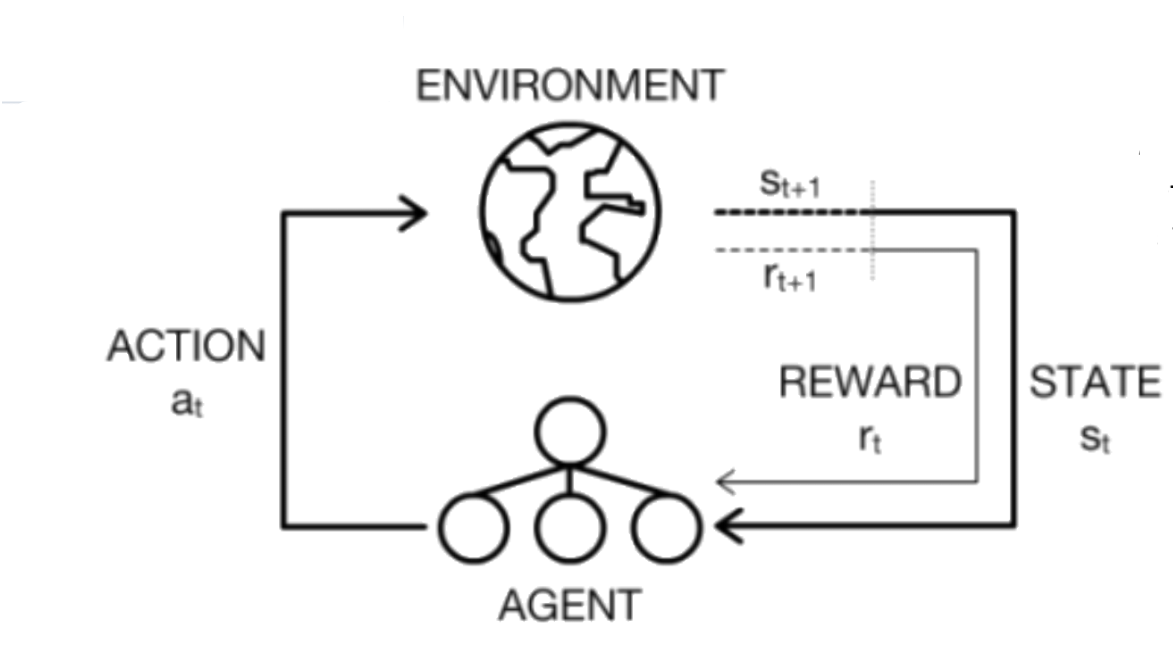
\includegraphics[width=.6\linewidth]{rl_1.png}
\end{center}
\end{frame}


\begin{frame}{Reinforcement Learning}
\begin{center}
	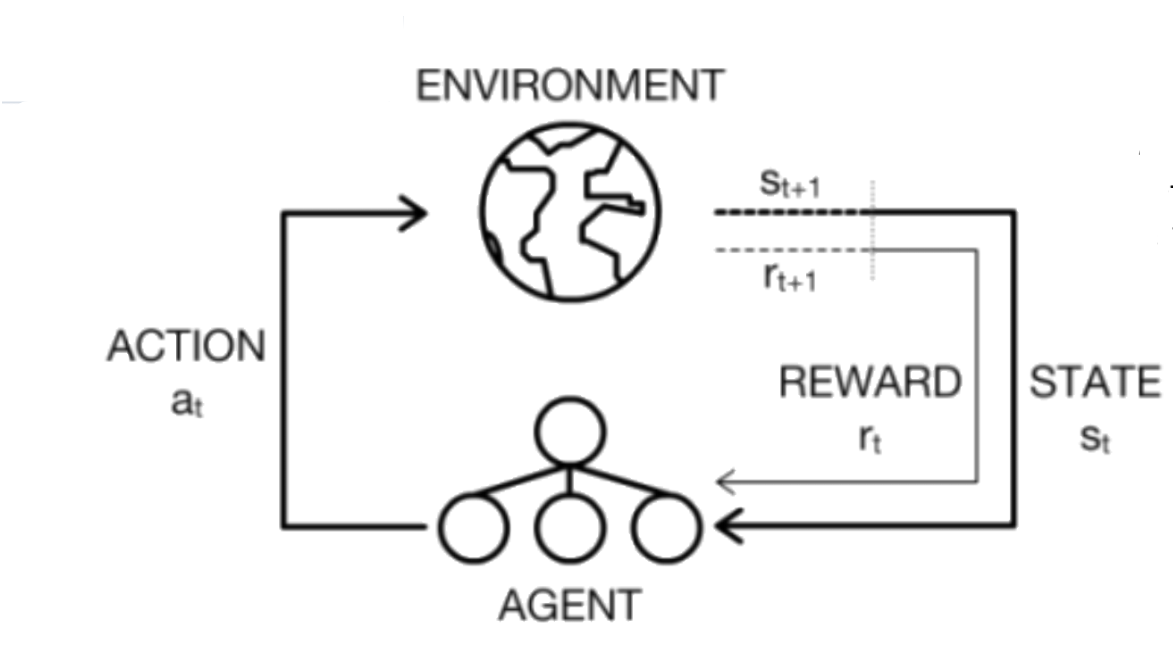
\includegraphics[width=.4\linewidth]{rl_1.png}
\end{center}
\begin{itemize}
	\item  $s_t$ --- состояние среды (state);
	\item  $a_t$ --- действия агента (action);
	\item  $r_t$ --- награда (reward) за действие;
\end{itemize}
\end{frame}


\begin{frame}{Reinforcement Learning}
\begin{center}
	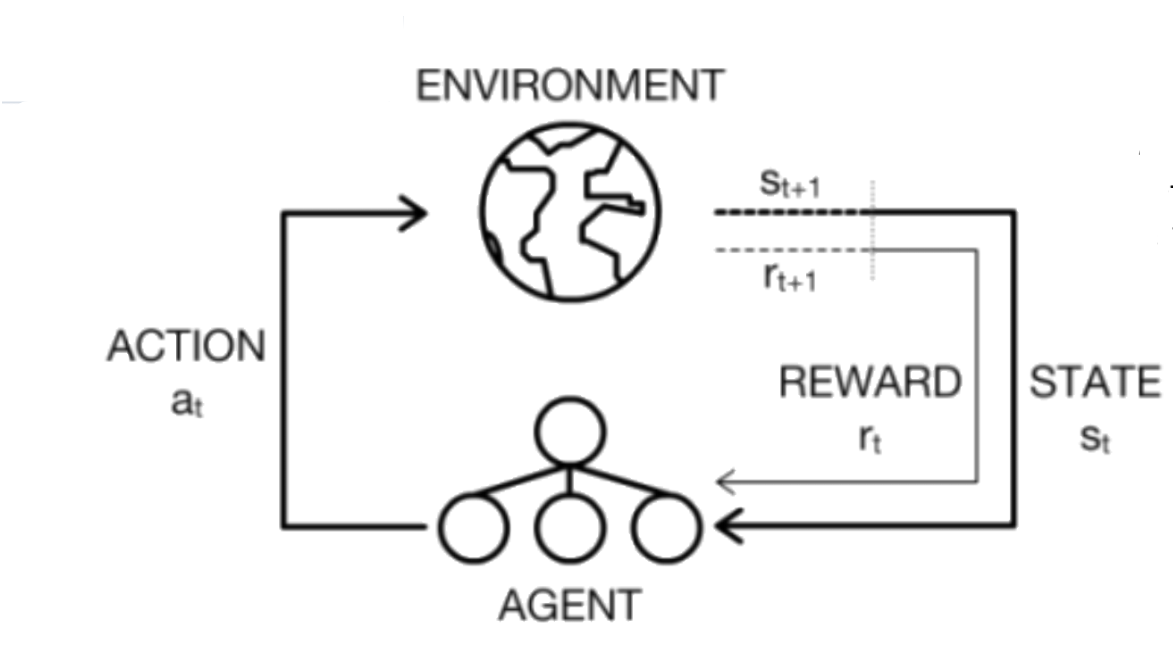
\includegraphics[width=.4\linewidth]{rl_1.png}
\end{center}
\begin{itemize}
	\item  $p(a \mid s)$ --- policy function, выводит вероятность действия в конкретном состоянии так, чтобы вероятность действия, максимизирующего reward была наибольшей 
	\item  $v(s)$ --- value function, по state выдаёт оценку всех будущих reward;
	\item  $Q(s,a)$ --- Q-function, сообщает reward для действия $a$ в состоянии $s$.
\end{itemize}
\end{frame}


\begin{frame}{Reinforcement Learning}
\begin{wideitemize}
\item \alert{Идея:} мы пытаемся выразить действия агента с помощью различных функций. Если мы пытаемся каждую функцию представить в виде нейросетки, мы входим в зону deep reinfircment learning. 

\item В зависимости от того, какую функцию мы оптимизируем, получаем разные алгоритмы 

\item В примере ниже мы будем максимизировать policy function (policy gradient algorithm), после будем заниматься оптимизацией Q-функции (Q-learning)
\end{wideitemize}
\end{frame}



\begin{frame}{Пример: игра в Pong}
\begin{center}
	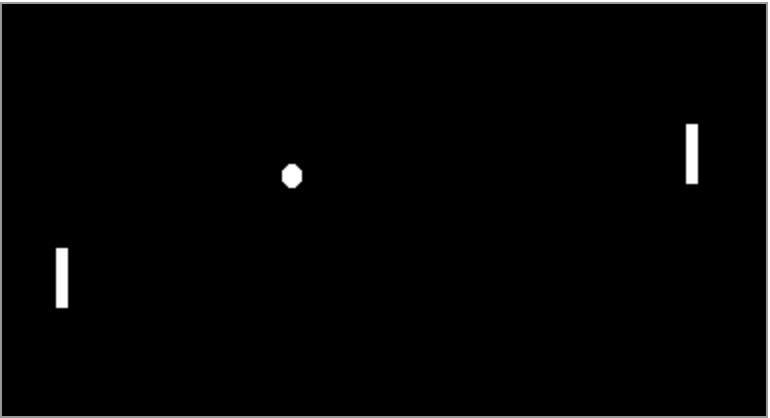
\includegraphics[width=.8\linewidth]{pong.png}
\end{center}
\vfill
{\color{blue}  \url{http://karpathy.github.io/2016/05/31/rl/}}
\end{frame}


\begin{frame}{Пример: игра в Pong}
\begin{center}
	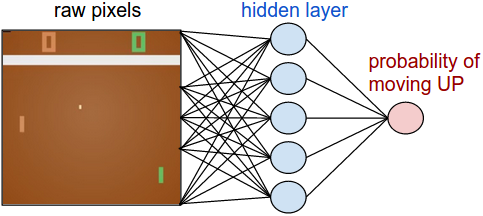
\includegraphics[width=.6\linewidth]{pong_NN.png}
\end{center}
\vfill
{\color{blue}  \url{http://karpathy.github.io/2016/05/31/rl/}}
\end{frame}


\begin{frame}{Пример: игра в Pong}
\begin{wideitemize}
	\item  Хотим натренировать белую палку выигрывать! 
	
	\item  Состояние $s_t$ --- пиксели экрана
	
	\item Мы хотим обучить нейросеть с одним скрытым слоем, которая по текущему дифу из пикселей предсказывать вероятность движения вверх или вниз 
	
	\item Сеть сама пытается разобраться как правильно играть в эту игру на основе разницы между текущим и предыдущим кадром 
\end{wideitemize}
\end{frame}


\begin{frame}{Пример: игра в Pong}
\begin{center}
	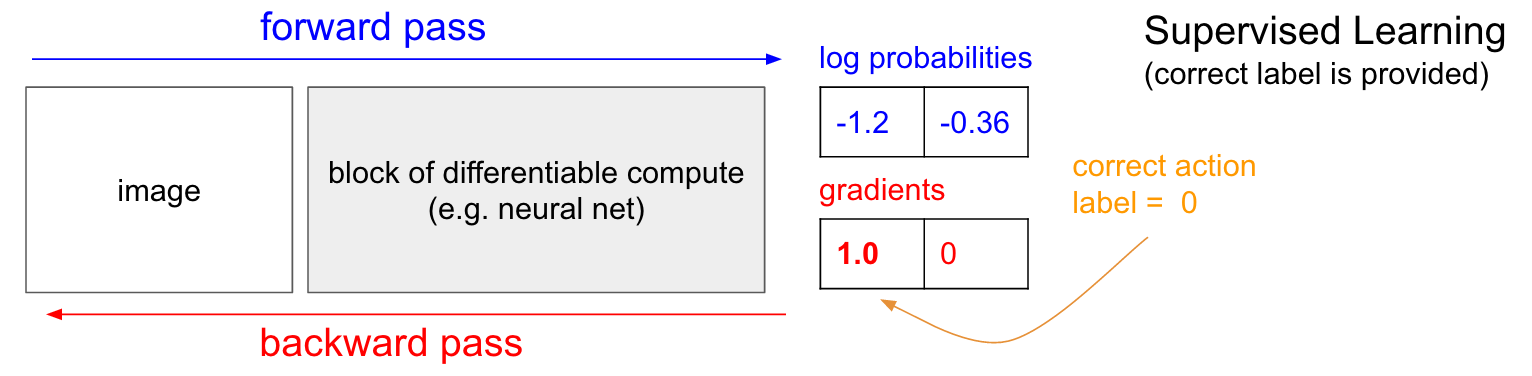
\includegraphics[width=.8\linewidth]{pong_label.png}
\end{center}
\vfill \pause 
\begin{center}
	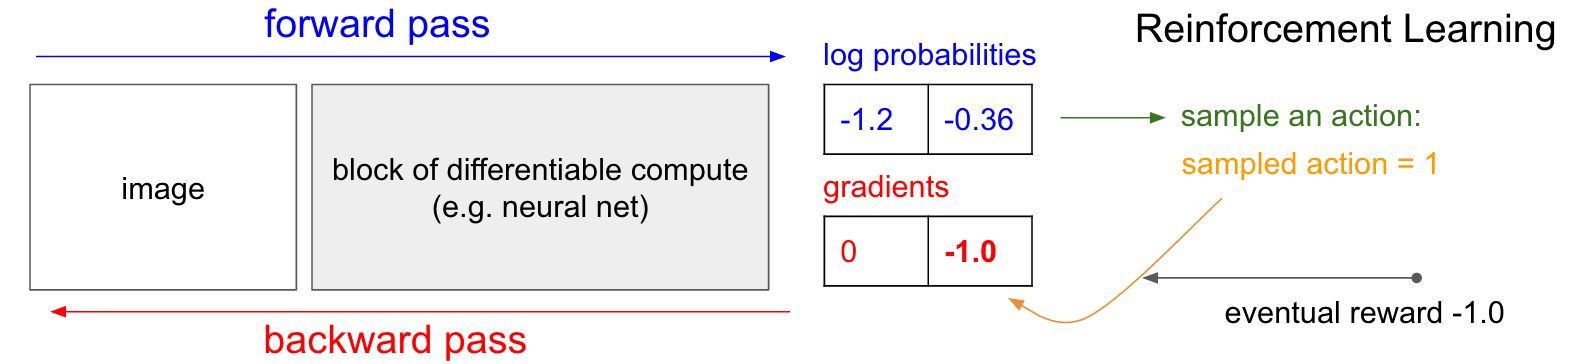
\includegraphics[width=.8\linewidth]{pong_sample.png}
\end{center}
\end{frame}


\begin{frame}{Пример: игра в Pong}
\begin{wideitemize}
	\item   Если бы мы учили обычную сетку, у нас был бы вектор правильных ответов для каждого действия, и мы бы делали backpropagation 
	
	\item  На деле мы знаем результат после многих шагов
	
	\item  Будем передавать вместо таргета то, что произошло на самом деле для последовательности действий 
\end{wideitemize}
\end{frame}


\begin{frame}{Пример: игра в Pong}
\begin{center}
	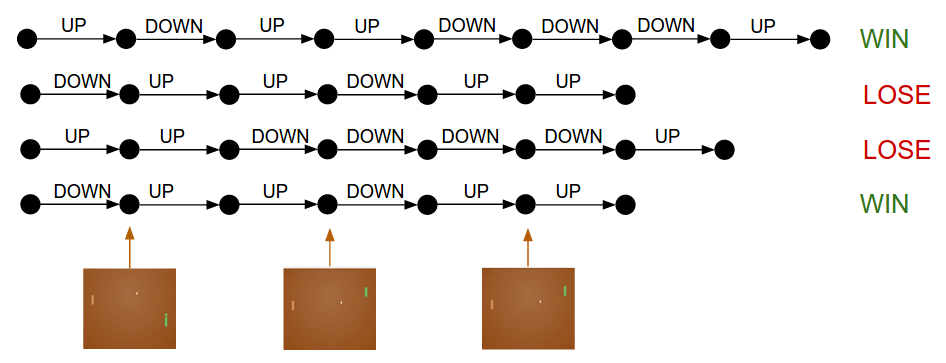
\includegraphics[width=.8\linewidth]{pong_backprop.png}
\end{center}
\end{frame}


\begin{frame}{Почему это работает?}
\begin{wideitemize}
	\item   Пусть $p(a \mid s, \theta)$ --- вероятность действия $a$ в состоянии $s$, описываемая параметрами $\theta$, а $f(a)$ --- награда от действия $a$
	\item Мы хотим двигать веса $\theta$ так, чтобы средняя награда $E_a [ f(a)]$ увеличивалась
	\item Добиться этого можно с помощью градиентного спуска
\end{wideitemize}
\end{frame}


\begin{frame}{Почему это работает?}
\begin{equation*}
\begin{aligned}
\nabla_{\theta} E_a [f(a)] & = \nabla \sum_a p(a) \cdot f(a) = \\
& = \sum_{a} \nabla_{\theta} p(a) \cdot f(a) = \\
& = \sum_{a} p(a) \cdot \frac{\nabla_{\theta} p(a)}{p(a)} \cdot f(a) = \\
& = \sum_{a} p(a) \cdot \nabla_{\theta} \ln p(a) \cdot f(a) = \\
& = E_a [ f(a) \cdot \nabla_{\theta} \ln p(a) = - logloss \\
\end{aligned}
\end{equation*}
\end{frame}


\begin{frame}{Какой бывает награда}
\begin{center}
	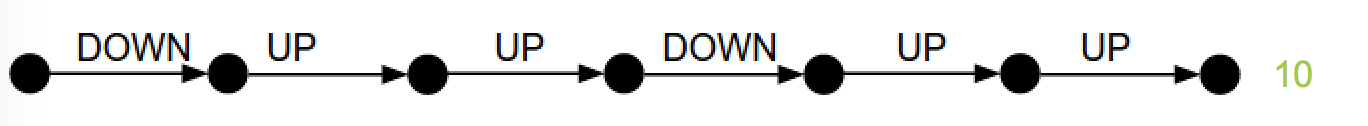
\includegraphics[width=.7\linewidth]{states.png}
\end{center}
\begin{itemize}
	\item В примере выше мы получали награду $r$ за какую-то последовательность действий
	\item Можно определить награду так, что мы её получаем на каждом шаге $r_t$
\end{itemize}
\begin{center}
	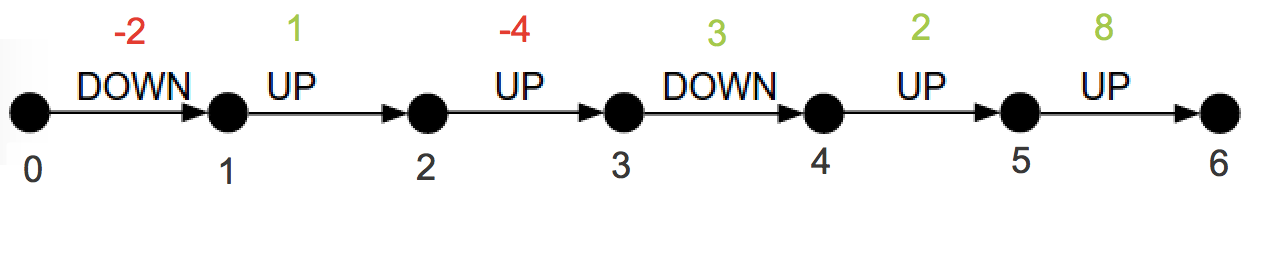
\includegraphics[width=.7\linewidth]{states_1.png}
\end{center}
\end{frame}


\begin{frame}{Какой бывает награда}
\begin{center}
	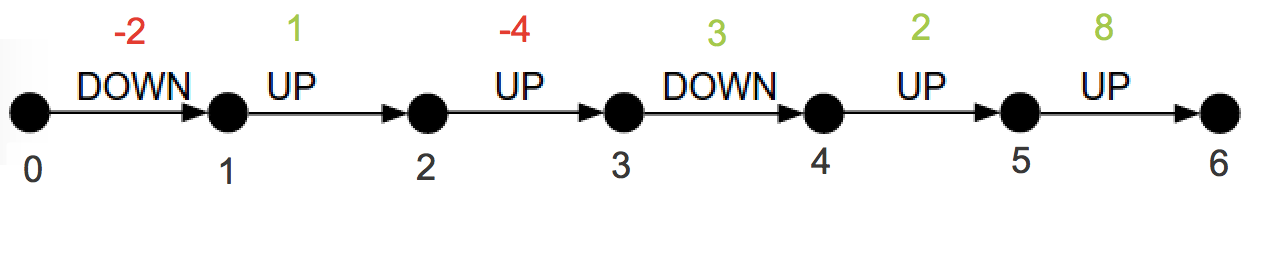
\includegraphics[width=.7\linewidth]{states_1.png}
\end{center}
\begin{equation*}
\begin{aligned}
&R_0 = r_0 + r_1 + r_2 + \ldots + r_{h}  & \qquad  R_1 = r_1 + r_2 + \ldots + r_{h} & \ldots \\
&R_0 = r_0 + \gamma \cdot r_1 + \gamma \cdot r_2 + \ldots +  \gamma^h \cdot r_{h}  & \qquad  R_1 = r_1 + \gamma \cdot r_2 + \ldots + \gamma^{h-1} \cdot r_{h} & \ldots \\
\end{aligned} 
\end{equation*}
\end{frame}

\begin{frame}{Какой бывает награда}

\alert{Фактор дисконтирования $\gamma$} нужен, чтобы очень далёкое будущее влияло на текущее состояние сети не так сильно, как в недалёком. Когда мы просим сеть разобраться с ближайшим будущим, ей легче разобраться в ситуации и обучение стабильнее. 
\end{frame}




% \begin{transitionframe}
%	\begin{center}
%		\Huge  История автоперевода
%	\end{center}
%\end{transitionframe}
%
%\begin{frame}
%\begin{center}
%	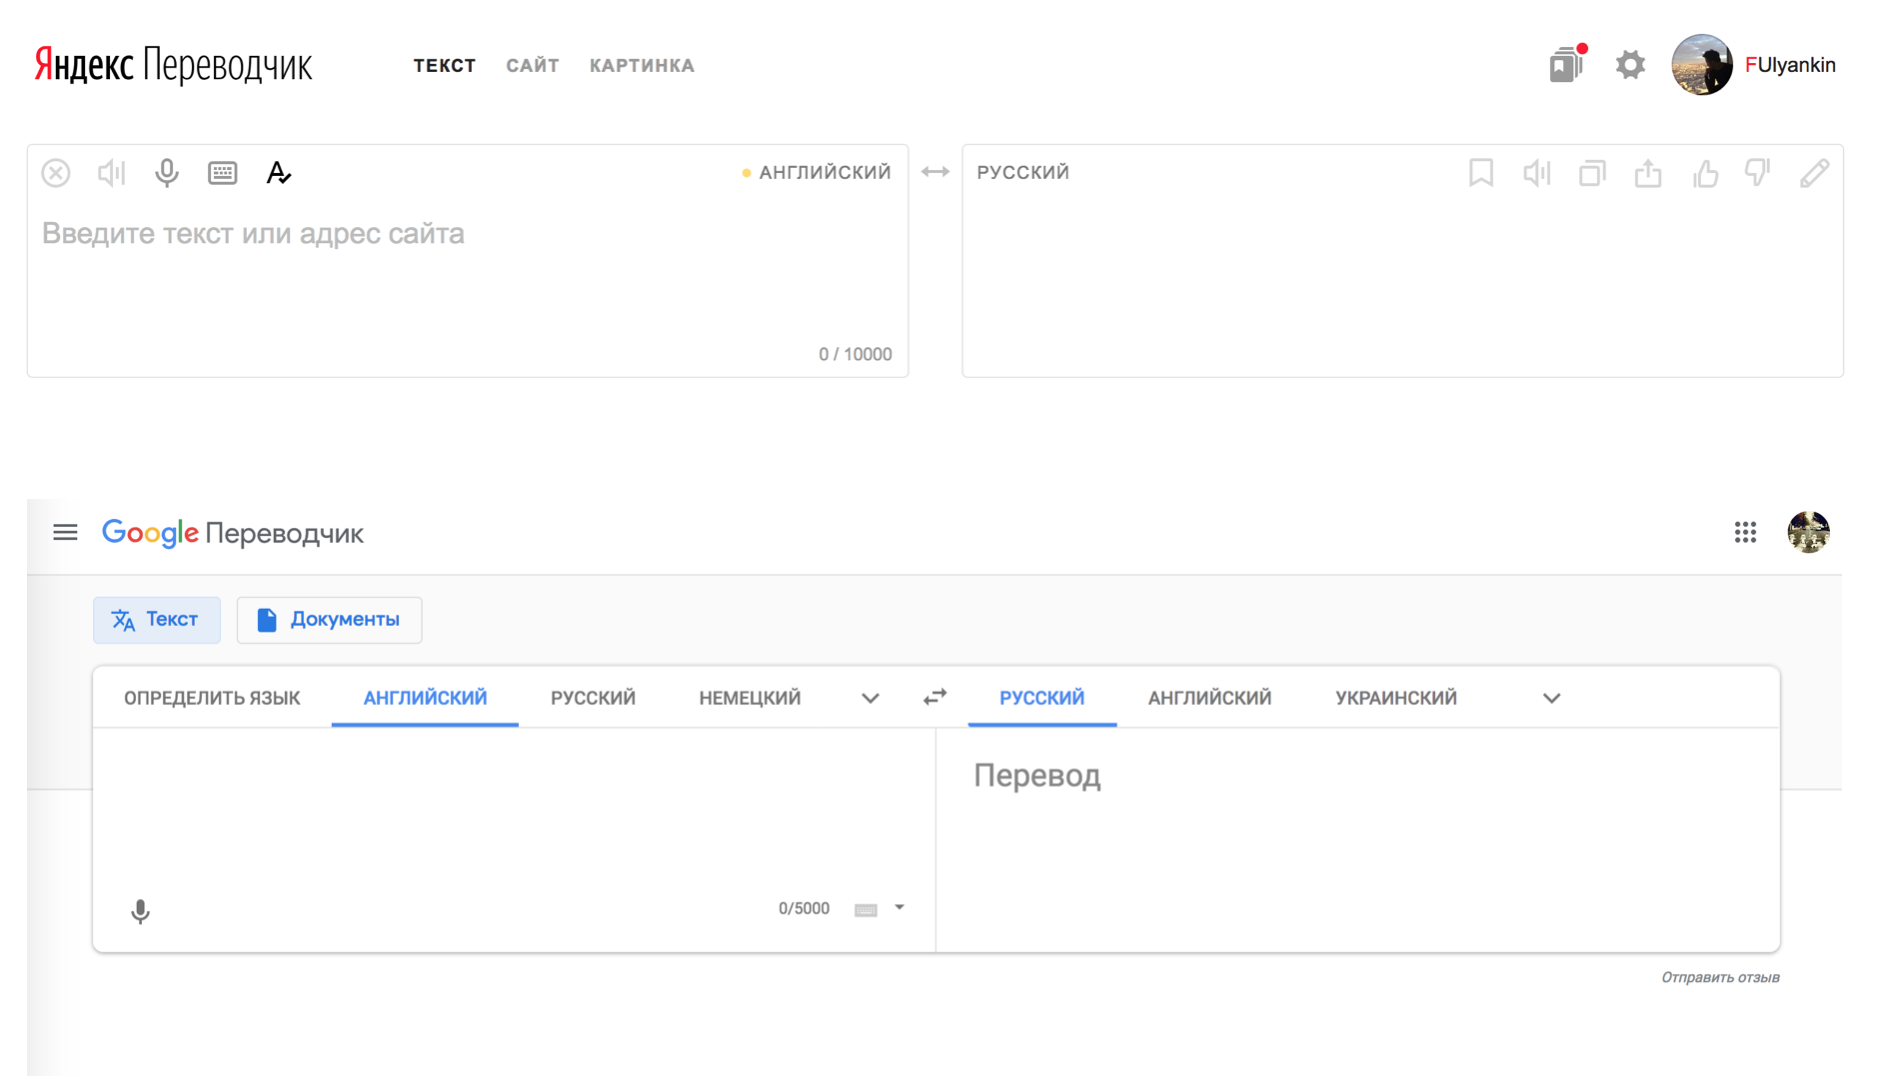
\includegraphics[width=.9\linewidth]{ya_go.png}
%\end{center}
%\end{frame}
%
%\begin{frame} {Когда и кто захотел} 
%\begin{wideitemize}
%	\item   Холодная война, 1954 год. США и СССР хотят получить машину для автопереводов 
%	\item   Джорджтаунский эксперимент. Перевод компом IBM 60 предложений с перфокарт $\Rightarrow$ приток денег в исследования
%	\item  В СССР аналогичный эксперимент 
%	\item  В обоих государствах все предложения для перевода тщательно подобраны и оттестированы :(
%\end{wideitemize}
%\end{frame}
%
%\begin{frame} {Когда и кто захотел} 
%\begin{wideitemize}
%	\item   Учёные обещают, что в течение ближайших 5 лет задача машинного перевода будет решена. 
%	\item Через 12 лет, в 1966 американский комитет ALPAC публикует отчёт, в котором называет машинный перевод дорогим, неточным и бесперспективным
%\end{wideitemize}
%\end{frame}
%
%\begin{frame} {Перевод на основе правил (Rule-based machine translation, RBMT)} 
%\begin{wideitemize}
%	\item  Получает интенсивное развитие в 1970-х годах
%	\item  Словари + попытка посмотреть на то как работают лингвисты и вбить какие-то паттерны в компьютер (существительные оканчиваются на а-я и тп) 
%	\item  Бывает разных видов 
%\end{wideitemize}
%\end{frame}
%
%\begin{frame} {RBMT)} 
%\begin{wideitemize}
%	\item  \alert{Дословный перевод (Direct Machine Translation):} делим текст по словам, переводим каждое, правим каждое слово в соответствии с накопленными правилами  (окончания, падежи и тп). Правила придумывают лингвисты.
%	\item  \alert{Трансферные системы (Transfer-based Machine Translation):} сначала выделяем синтаксические конструкции (сказуемые, подлежащие и тп), понимаем как слова надо переставить, а потом уже переводим.
%\end{wideitemize}
%\end{frame}
%
%\begin{frame} {Эти типы стали есть на складе} 
%\begin{wideitemize}
%	\item  Придумывать правила вручную - сложно
%	\item  Огромное количество исключений 
%	\item  Омонимия (разный смысл одних и тех же слов в зависимости от контекста) 
%	\item  RBMT системы за годы холодной войны вышли на пик и успешно умерли, сегодня они не используются нигде 	
%\end{wideitemize}
%\end{frame}
%
%\begin{frame} {Example based machine translation (EBMT)} 
%\begin{wideitemize}
%	\item   Япония, 1984 г. 
%	\item   Зачем каждый раз переводить заново? Давайте переиспользовать! 
%	\item   Впервые возникла идея просто скармливать компьютеру существующие данные, а не придумывать правила
%\end{wideitemize}
%\begin{center}
%	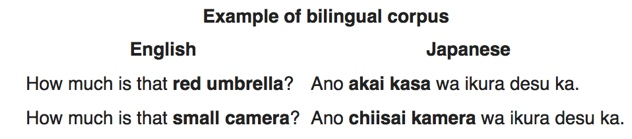
\includegraphics[width=.6\linewidth]{ex_tr_1.jpg}
%\end{center}
%\end{frame}
%
%\begin{frame} {Statistical machine translation (SMT)} 
%\begin{wideitemize}
%	\item   IBM, 1990 г. 
%	\item   Берём корпус параллельных текстов, смотрим как часто слово house переводится как дом, строение, постройка, так и переводим! 
%	\item   Работало лучше, чем всё что было до этого
%\end{wideitemize}
%\end{frame}
%
%\begin{frame} {SMT} 
%\begin{center}
%	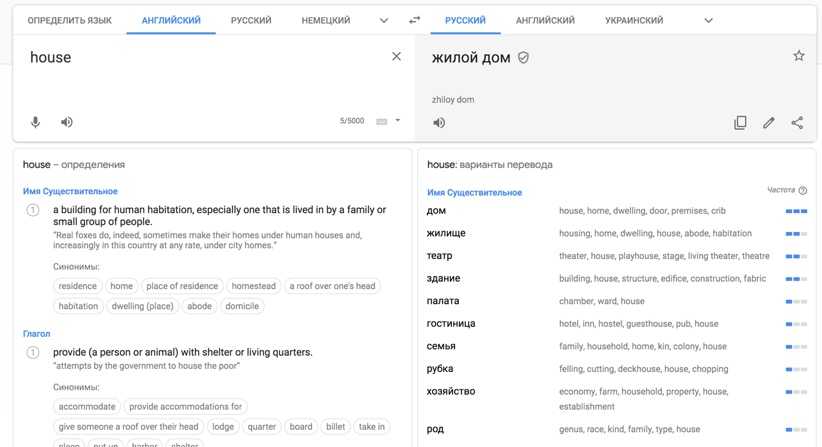
\includegraphics[width=.8\linewidth]{ggl.jpg}
%\end{center}
%\end{frame}
%
%\begin{frame} {Word-based SMT} 
%\begin{wideitemize}
%	\item   Начали конечно же со статистического перевода по отдельным словам
%	\item   Пример реализации на python: {\color{blue} \url{https://github.com/shawa/IBM-Model-1}}
%	\item   Дальше попробовали также по статистике переставлять слова, добавлять недостающие артикли
%	\item  Всё ещё много проблем с омонимией и согласованностью слов в предложениях
%\end{wideitemize}
%\end{frame}
%
%\begin{frame} {Phrase-based SMT} 
%\begin{wideitemize}
%	\item   Word-based SMT был основан на мешке слов, тут подмешали N-граммы 
%	\item   C 2006 года этот подход использовали абсолютно все
%	\item   Так продолжалось до 2016 года
%	\item  В 2016 году Google перевернул игру: {\color{blue} \url{https://ai.googleblog.com/2016/09/a-neural-network-for-machine.html}}
%\end{wideitemize}
%\end{frame}
%
%\begin{frame}
%\begin{center}
%	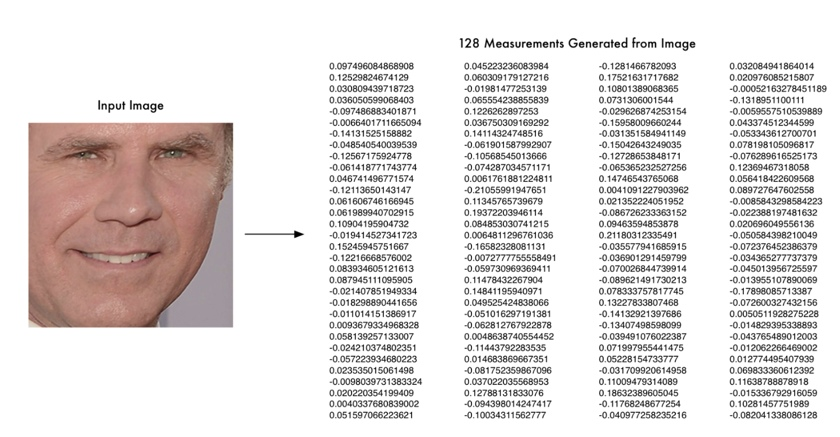
\includegraphics[width=.8\linewidth]{img_vec.jpg}
%\end{center}
%\end{frame}
%
%\begin{frame}
%\begin{center}
%	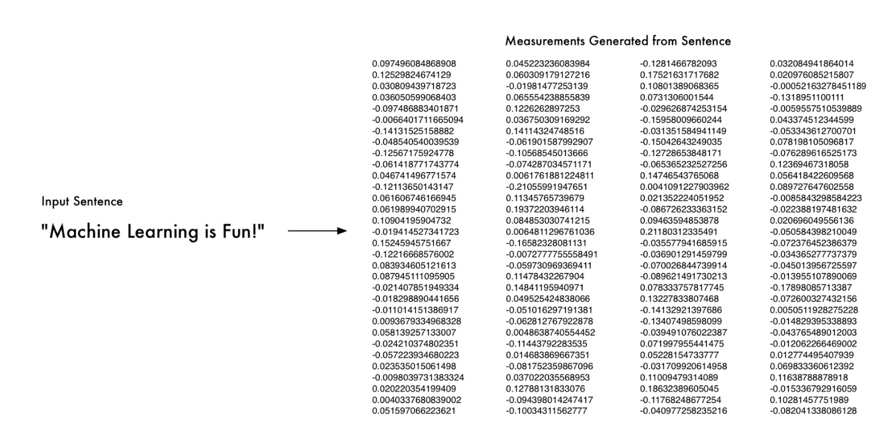
\includegraphics[width=.8\linewidth]{word_vec.jpg}
%\end{center}
%\end{frame}
%
% \begin{transitionframe}
%	\begin{center}
%		\Huge  Текст + картинка
%	\end{center}
%\end{transitionframe}
%
%\begin{frame}{Генерация подписи по картинке}
%\begin{center}
%	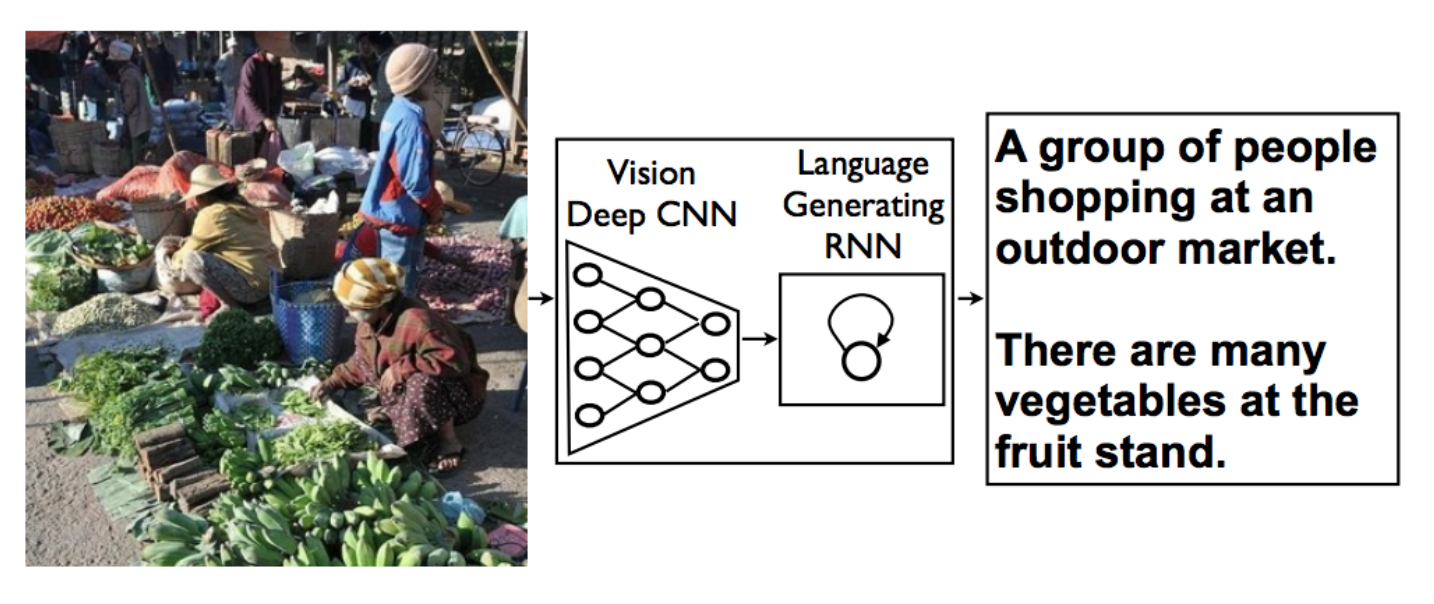
\includegraphics[width=.7\linewidth]{imgentext.png}
%\end{center}
%\end{frame}
%
%
%\begin{frame}{Генерация подписи по картинке}
%\begin{center}
%	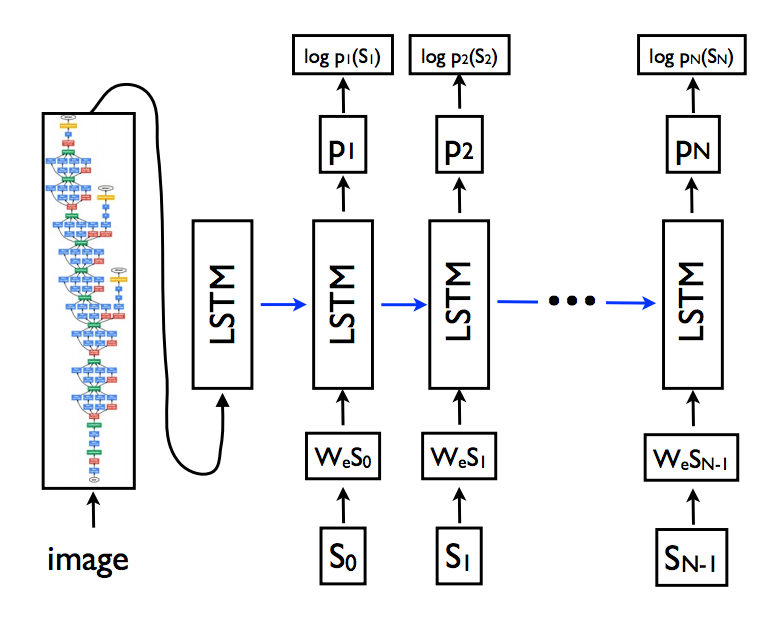
\includegraphics[width=.5\linewidth]{pictext.png}
%\end{center}
%
%\url{https://arxiv.org/abs/1411.4555}
%\end{frame}
%
%
%\begin{frame}{Генерация подписи по картинке}
%\begin{center}
%	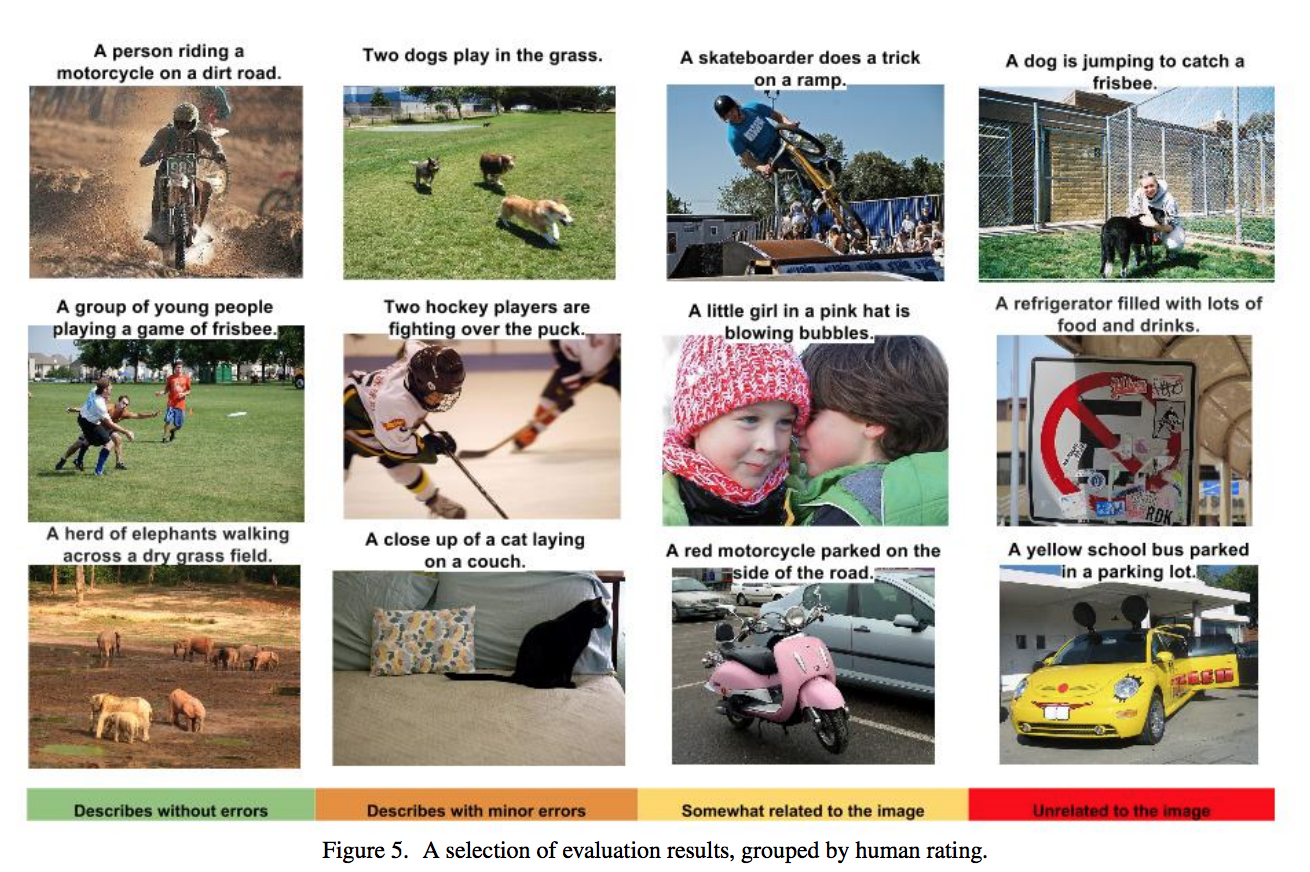
\includegraphics[width=.7\linewidth]{pic_text.png}
%\end{center}
%\end{frame}
%
%
%\begin{frame}{Генерация подписи по картинке}
%\begin{center}
%	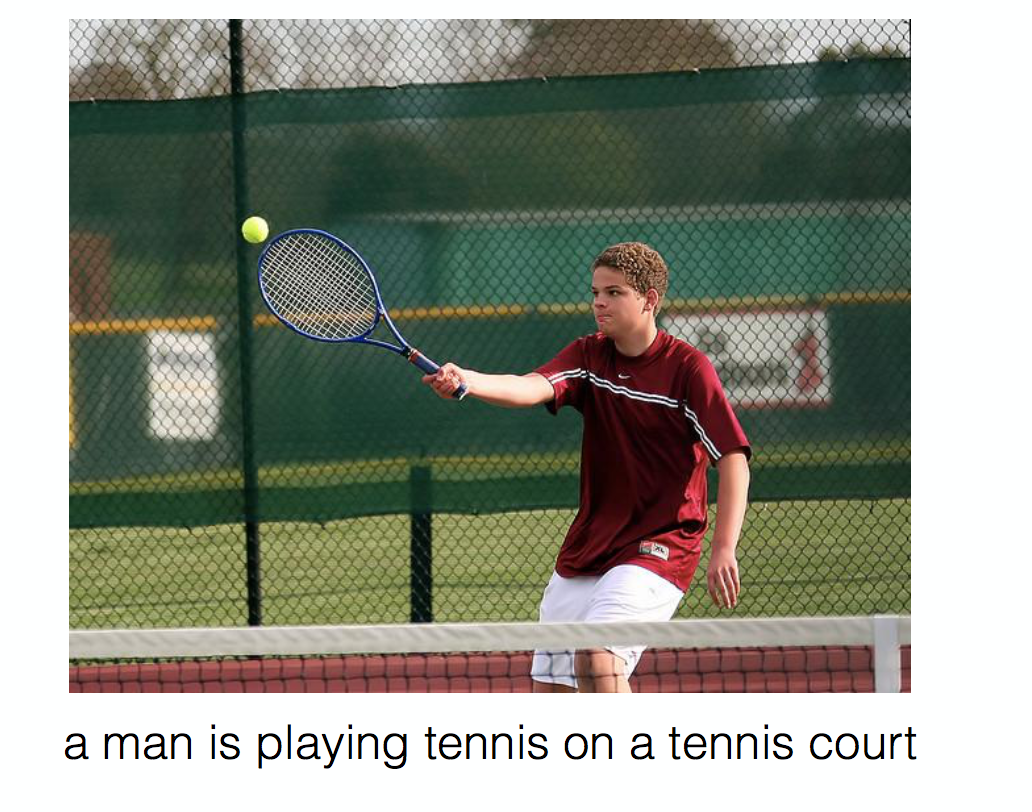
\includegraphics[width=.6\linewidth]{pic_text_ex1.png}
%\end{center}
%\end{frame}
%
%
%\begin{frame}{Генерация подписи по картинке}
%\begin{center}
%	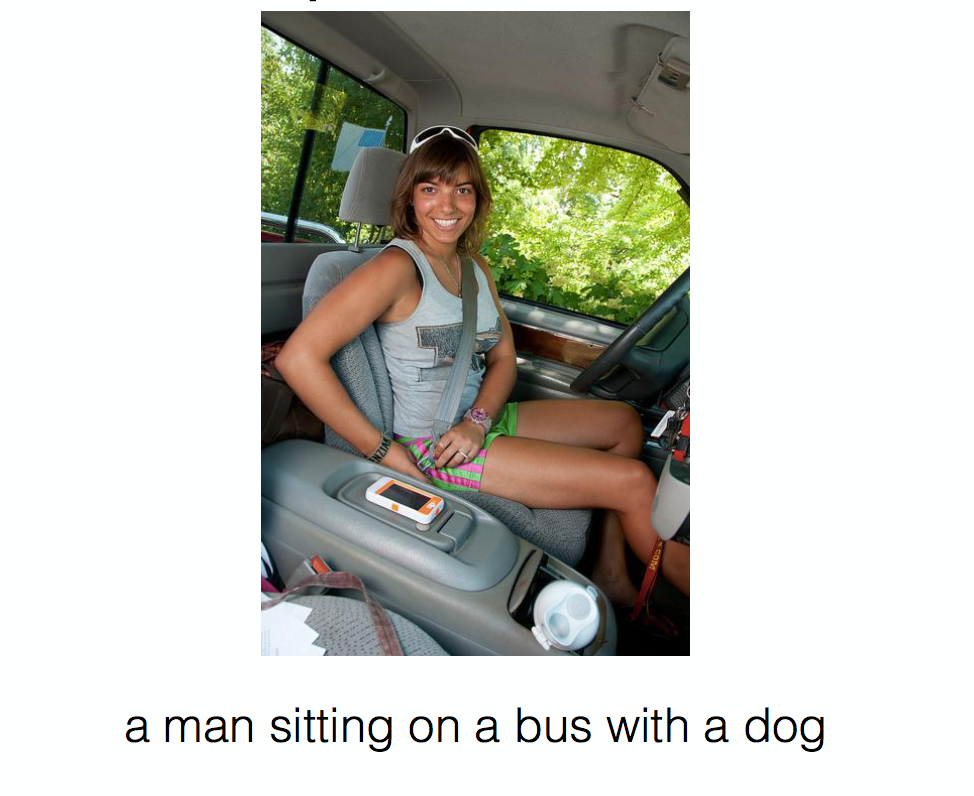
\includegraphics[width=.6\linewidth]{pic_text_ex2.png}
%\end{center}
%\end{frame}
%
%
%\begin{frame}{Генерация подписи по картинке}
%\begin{center}
%	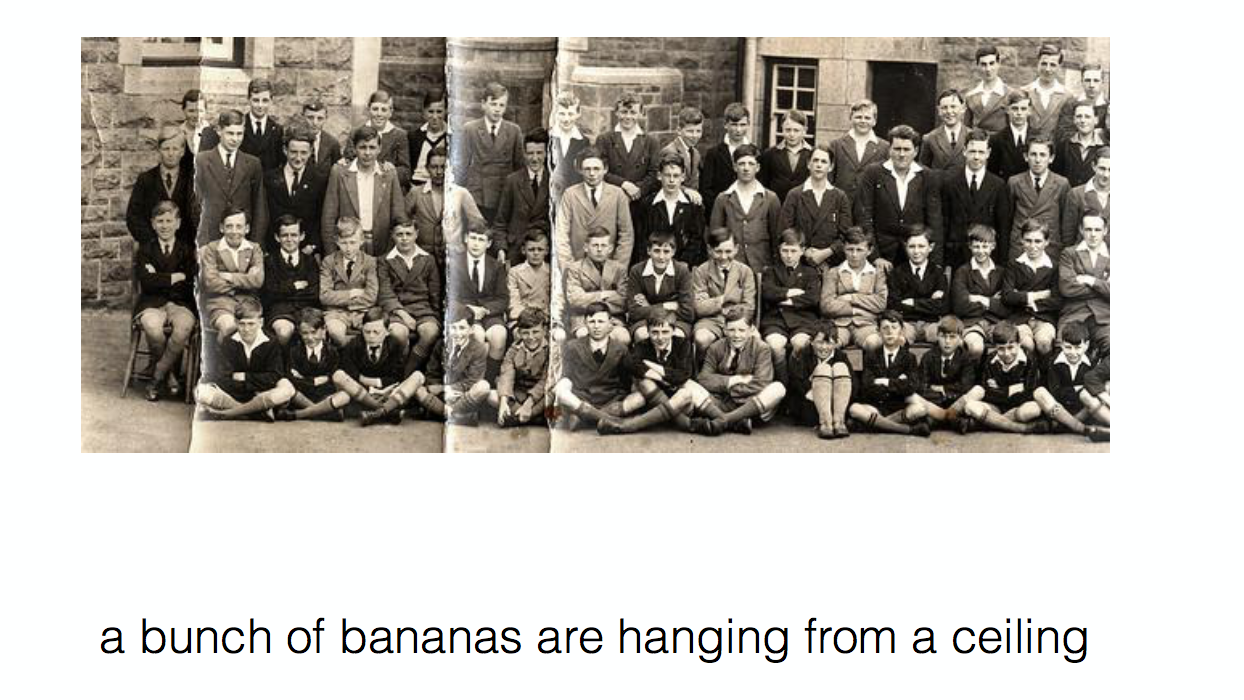
\includegraphics[width=.8\linewidth]{pic_text_ex3.png}
%\end{center}
%\end{frame}
%
%
%\begin{frame}{Архитектура}
%\begin{center}
%	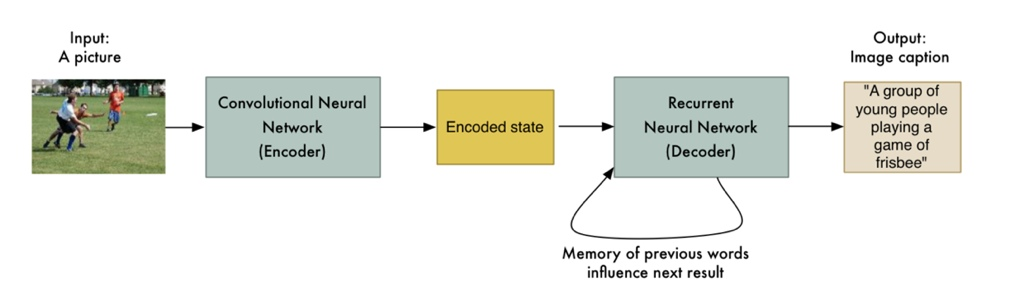
\includegraphics[width=.95\linewidth]{pic_text_nn.jpg}
%\end{center}
%\end{frame}
%
%
% \begin{transitionframe}
%	\begin{center}
%		\Huge  Автопереводчик 
%	\end{center}
%\end{transitionframe}
%
%
%\begin{frame}{Автокодировщик для текстов}
%\begin{center}
%	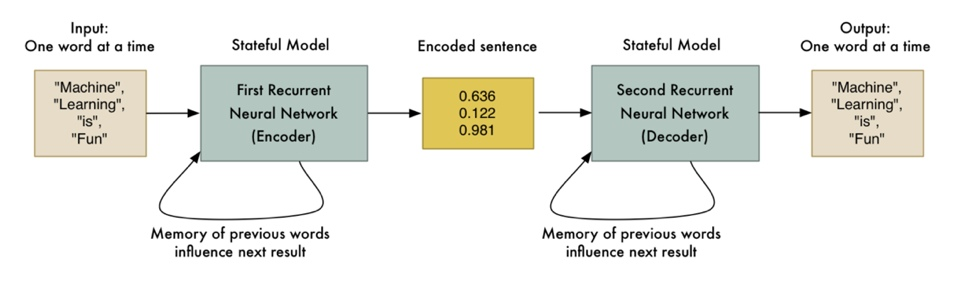
\includegraphics[width=.95\linewidth]{text_autocod.jpg}
%\end{center}
%\end{frame}
%
%
%\begin{frame}{Переводчик}
%\begin{center}
%	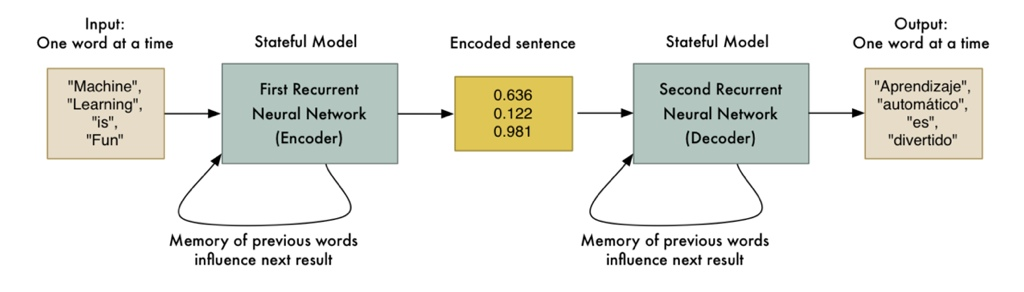
\includegraphics[width=.95\linewidth]{text_trans.jpg}
%\end{center}
%\end{frame}
%
%
%\begin{frame} {Переводчик} 
%\begin{wideitemize}
%	\item  Архитектуры переводчиков очень разные
%	\item  Поначалу это были RNN, после перешли на многослойные двунаправленные LSTM 
%	\item  Сегодня есть ещё куча разных штук, которыми пичкают автопереводчики
%	\item  Например, пробуют разные виды эмбедингов, добавляют модели с вниманием для согласования контекста 
%\end{wideitemize}
%\end{frame}
%
%
%\begin{frame} {Google vs Yandex} 
%\begin{wideitemize}
%	\item  Переводчик Google - нейросетевой 
%	\item  Переводчик Yandex очень сильно от него отличается
%	\item  На коротких фразах нейросетевой перевод работает плохо, поэтому 
%	\item  Перевод идёт двумя способами: статистическим и нейросетевым, а после Catboost выбирает тот, который лучше подходит 
%\end{wideitemize}
%\end{frame}
%
%
%\begin{frame} {Ссылки} 
%\begin{wideitemize}
%	\item  Пресс-релиз Яндекса от 2017: {\color{blue} \url{https://yandex.ru/blog/company/kak-pobedit-mornikov-yandeks-zapustil-gibridnuyu-sistemu-perevoda}}
%	\item  	Статья Яндекса на хабре про историю автоперевода: {\color{blue} \url{https://habr.com/ru/company/yandex/blog/224445/}}
%\end{wideitemize}
%\end{frame}
%
%


\end{document}
